\documentclass{report}
\usepackage[utf8]{inputenc}
\usepackage{tabularx}
\usepackage{graphicx}
\usepackage{hyperref}
\usepackage{fixlatvian}
\usepackage[siunitx]{circuitikz}
\usepackage{circuitikz}
\usepackage{tikz}
\usepackage{amssymb}
\usepackage{amsmath}
\usepackage{latexsym}
\usepackage[section]{placeins}



\title{Vienkāršu elektrisku shēmu modelēšana}
\author{Druvis Ēriks Tulišs }
\date{May 2018}
\begin{document}

\maketitle

\chapter{Teorētiskā daļa}

\section{Teorētiskā ķēdes aprēķina noteikumi:}
    Apēķiniet spriegumus uz rezistoriem 1. attēlā dotajā shēmā. Sprieguma avota V1 sprieguma
    vērtību U (Voltos) izvēlieties daļskaitli, kas būtu Jūsu apliecības pēdējie trīs cipari dalīti ar
    10. R1 ir apliecības pēdējo 3 ciparu otrais numurs+1, R2 ir apliecības numura pēdējais cipars +1.

\begin{flushleft}
    Apliecības nr. - 141RMC192
\end{flushleft}

\section{Teorētiskais ķēdes aprēķins:}

\begin{flushleft}
    UR1=192/10=19.2V\\
    R1=9+1=10\\
    R2=2+1=3\\
\end{flushleft}

\section{Rezultātu tabula:}

\begin{tabular}{|c|c|}
    \hline
        $R_1$ & 10\\
    \hline
        $R_2$ & 3  \\
    \hline
        $V_1$ & 19.2  \\
    \hline
        $U_{R1}$ & 19.2  \\
    \hline
        $U_{R2}$ & 9.6 \\
    \hline
\end{tabular}

\section{Shēma, ko izmantos lab.d:}

\begin{center}
    \begin{circuitikz}[american voltages]
        \draw
            [fill] (4,5) circle (0.3ex) node [above] {2}
            [fill] (0,3.5) circle (0.3ex) node [left] {1}
            (0,0)   to[battery1, l = $V_1$] (0,5)
                    to[european resistor, l = $R_1$] (5,5)
                    to[european resistor, l = $R_2$] (5,0) -- (4,0)
                    to (0.5,0) -- (0,0)
            [fill] (5,0.5) circle (0.3ex) node [right] {0}
    \end{circuitikz}
\end{center}

\chapter{Praktsikā daļa}

\section{Darbs ar GEDA programmām}

    \subsection{Darbs ar gschem:}

        \begin{figure}[h]
            \centering
            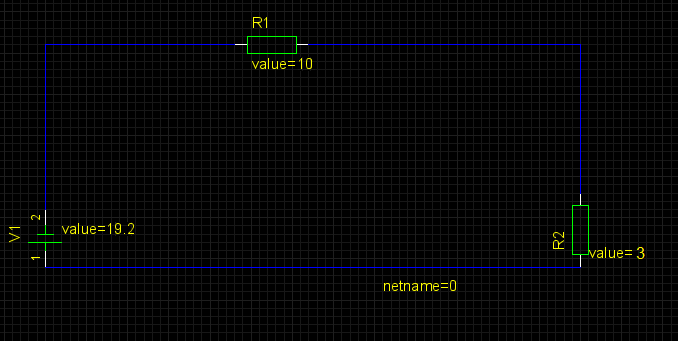
\includegraphics[width=.6\textwidth]{Lab.d/data/gEDA.png}
            \caption{gEDA shēma}
            \label{fig:my_label1}
        \end{figure}

    \subsection{Darbs ar gnetlist:}
    
        \begin{figure}[h]
            \centering
            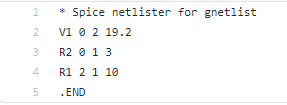
\includegraphics[\textwidth]{Lab.d/data/01.netlist.PNG}
            \caption{Rezultātu pārbaude ar gnetlist}
            \label{fig:my_label2}
        \end{figure}
    
    \subsection{Darbs ar ngspice:}
    
        \begin{figure}[h]
            \centering
            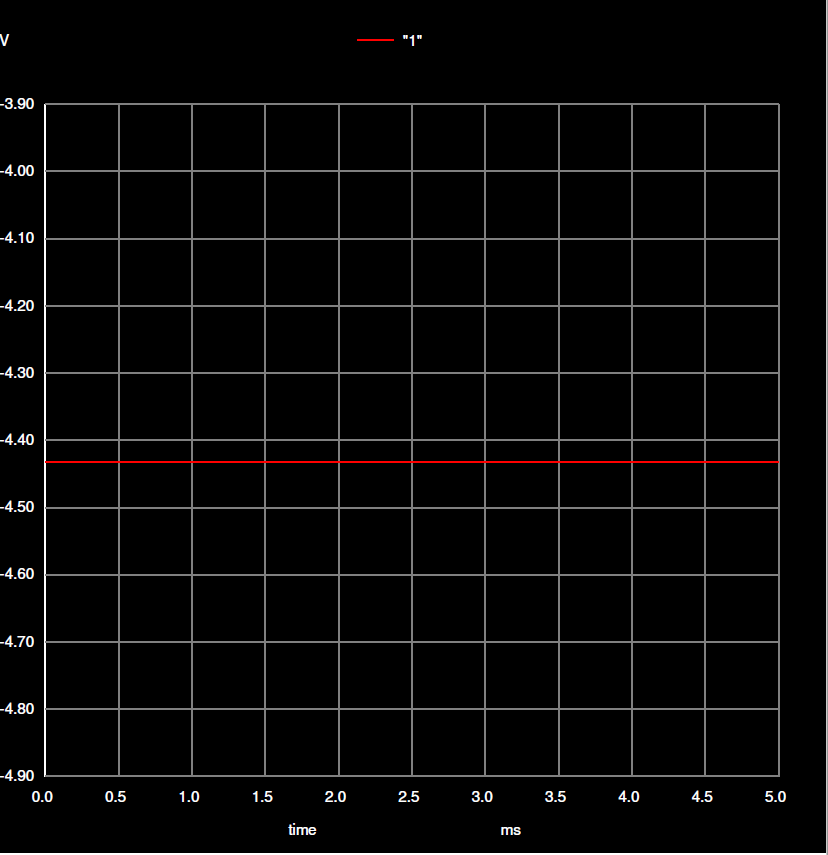
\includegraphics[width=.5\textwidth]{Lab.d/data/011.PNG}
            \caption{Ngspice iegūtais grafiks $R_1$}
            \label{fig:my_label3}
        \end{figure}
        
        \begin{figure}[h]
            \centering
            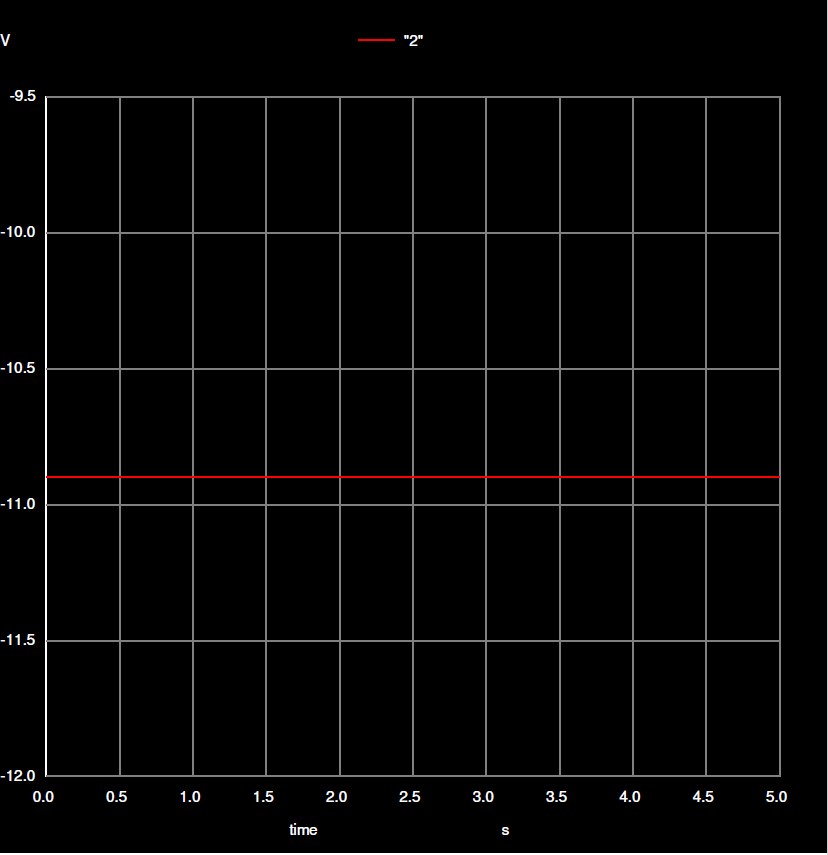
\includegraphics[width=.5\textwidth]{Lab.d/data/012.PNG}
            \caption{Ngspice iegūtais grafiks $R_2$}
            \label{fig:my_label4}
        \end{figure}
        
         \begin{flushleft}
            Diemžēl, kā redzams ir abos atēlos, manai shēmai snāca tikai taisnas līnijas nevis viļņveida grafiki.
        \end{flushleft}
       

\section{Darbs ar QUCS programmām}

    \subsection{Līdzstrāvas simulācijas (DC simulation) grafiku:}
        \begin{figure}[h]
            \centering
            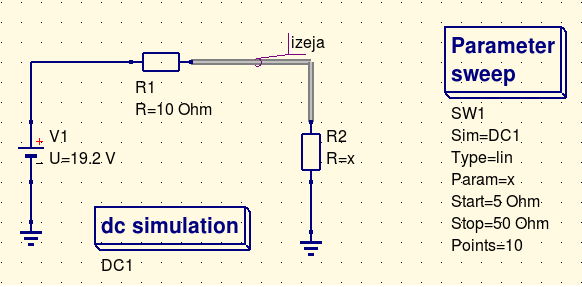
\includegraphics[width=.5\textwidth]{Lab.d/data/SHEMA.png}                \caption{QUCS simulācijas shēma}
            \label{fig:my_label5}
        \end{figure}

    \subsection{Sweep simulācijas grafiku ar tabulu:}
        \begin{figure}[h]
            \centering
            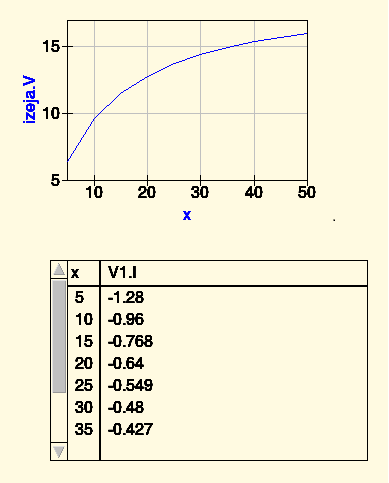
\includegraphics[width=.5\textwidth]{Lab.d/data/QUCS_TAB_GRAF.png}
            \caption{QUCS simulācijas grafiks ar tabulu}
            \label{fig:my_label6}
        \end{figure}    

\begin{thebibliography}{9}
    \bibitem{a_1}
        Māra Zālīte 
    \textit{"Pieci pirksti"}. 
        Latvija, Rīga: 20 lpp.

    \bibitem{a_2} 
        Nils Sakss  
    \textit{"Nāve - tās nav beigas"}. 
        Latvija, Rīga: 212 lpp.
\end{thebibliography}        
    
    
\end{document}
